\newpage
\section{Дифференциальное исчисление функций нескольких переменных}
\subsection{Дифференцируемые отображения}

\begin{definition}
    Пусть $f: E\rightarrow \R^m$, $E\subset \R^n$, $a\in \Int E$. Тогда $f$ \textit{дифференцируема в точке} $a$, если существует линейное отображение $T: \R^n \rightarrow \R^m$, т.ч. 
    
    $f(a + h) = f(a) + Th + o(\|h\|)$ при $h\rightarrow 0$.
\end{definition}

\begin{remark}
    Если $T$ существует, то оно определено однозначно. 
    
    Зафиксируем $h\in \R^n$, $t\in \R$: $f(a+th)=f(a)+T(th)+o(t)=f(a)+t\cdot Th + o(t)$.

    $Th = \lim\limits_{t\rightarrow 0}\frac{f(a+th)-f(a)}{t}$ (предел единственный $\Rightarrow$ значение $t$ на векторе определяется однозначно $\Rightarrow$ отображение определяется однозначно)
\end{remark}

\begin{definition}
    Матрица линейного оператора $T$ называется \textit{матрицей Якоби для отображения $f$} и обозначается $f'(a)$ (теперь матрица $f'$ – аналог производной).

    Линейный оператор $T$ называется \textit{дифференциалом функции $f$ в точке $a$} и обозначается $d_af$.
\end{definition}

\begin{remark}
    Дифференцируемость в точке $a$ влечет непрерывность в точке $a$.

    $f(a+h)=\underset{\rightarrow f(a)}{f(a)}+\underset{\rightarrow T0=0}{Th}+\underset{\rightarrow 0}{o(\|h\|)}$ при $h \rightarrow 0$
\end{remark}

\begin{remark}
    \textbf{Важный частный случай:} \textit{координатные функции}, из которых можно составить вектор.
    
    $m=1$, $f: E\rightarrow \R$, $E\subset \R^n$, $a\in \text{Int} E$.

    $f(a+h)=f(a)+Th+o(\|h\|)$ 

    Найдется такой $v\in \R^n: f(a+h)=f(a)+\langle v, h\rangle +o(\|h\|)$ при $h\rightarrow 0$. 

    \begin{definition}
        Этот вектор $v$ – \textit{градиент функции $f$} в точке $a$. Обозначается $\text{grad } f(a)$ или $\triangledown f(a)$ ($\triangledown$ – \textit{символ Набла}).    
    \end{definition}
\end{remark}

\begin{example}~
    \begin{enumerate}
        \item Постоянное отображение $f$ дифференцируемо во всех точках, $T=0$.
        \item Линейное отображение: $f(a+h)=f(a)+f(h)$, $T=f$.

        Матрица Якоби – матрица этого отображения $f$.
    \end{enumerate}
\end{example}

\begin{theorem}
    Пусть $f: E\rightarrow \R^m$, $E\subset \R^n$, $a\in \Int E$, $f=\begin{pmatrix}
        f_1  \\ \vdots \\ f_m
    \end{pmatrix}$, где $f_1, ..., f_m: E\rightarrow \R$ (\textit{координатные функции}). Тогда $f$ дифференцирема в точке $a\Leftrightarrow f_j$  дифференцируема в точка $a$ $\forall j=1, ..., m$.
\end{theorem}

\begin{proof}~
    \begin{enumerate}
        \item[$\Rightarrow$.] $f(a+h)=f(a) + Th + \alpha (h)\cdot \|h\|$, где $\alpha(h)\underset{h\rightarrow 0}{\rightarrow}0$.

         $f_j(a+h)=f_j(a) + T_jh + \alpha_j (h)\cdot \|h\|$, где $T_jh$ – это $j$-ая координата $Th$, $\alpha_j(h)$ – $j$-ая координата $\alpha(h)$.

         $|\alpha_j(h)|\leq \sqrt{\alpha_1(h)^2+...+\alpha_m(h)^2}=\|\alpha(h)\|\rightarrow 0$.

         \item[$\Leftarrow$.] $f_j(a+h)=f_j(a) + T_jh + \alpha_j (h)\cdot \|h\|$, составим из них равенство для векторов:

         $\alpha(h)=\begin{pmatrix}
             \alpha_1(h) \\ \vdots \\ \alpha_m(h)
         \end{pmatrix}$ и надо доказать, что $\alpha (h) \underset{h\rightarrow 0}{\rightarrow}0$: 
         
         $\|\alpha(h)\|= \sqrt{\alpha_1(h)^2+...+\alpha_m(h)^2}\leq \|\alpha_1(h)^2\|+...+\|\alpha_m(h)^2\| \underset{h\rightarrow 0}{\rightarrow}0$
    \end{enumerate}
\end{proof}

\begin{corollary}
    Матрица Якоби $f$ – матрица, составленная из градиентов координатных функций: $f'(a)=\begin{pmatrix}
             \triangledown f_1(a) \\ \vdots \\ \triangledown f_m(a)
         \end{pmatrix}$.
\end{corollary}

\begin{definition}
    Пусть $f: E\rightarrow \R$, $E\subset \R^n$, $a\in \Int E$, $h\in \R^n$ – единичный вектор. Тогда $\partialderivative{f}{h}(a):=\lim\limits_{t\rightarrow 0}\frac{f(a+th)-f(a)}{t}$ – \textit{производная $f$ по направлению $h$ в точке $a$}.
\end{definition}

\begin{remark}~
    \begin{enumerate}
        \item $\frac{\partial f}{\partial h}(a)=d_af(h)=\langle\triangledown f(a), h\rangle$.
        \begin{proof}

            Зафиксируем единичный $h\in \R^n$.
            
            По определению дифференцируемости $f$: $f(a+h)=f(a) + t\cdot Th + \alpha (th)\cdot \|h\|\Leftrightarrow f(a+th)-f(a)=Th +\alpha (h)$

            $\partialderivative{f}{h}(a)=\lim\limits_{t\rightarrow 0}\frac{f(a+th)-f(a)}{t} =\lim\limits_{t\rightarrow 0}\frac{t\cdot Th + \alpha (th)}{t\cdot \|h\|}=Th=d_fa$ (разделили на $\|h\|=1$)

            Второе равенство – определение градиента.
        \end{proof}
        \item Пусть $g: (-\delta, \delta)\rightarrow \R$, $g(t):= f(a+th)$. 
        
        Тогда $\frac{\partial f}{\partial h}(a)=\lim\limits_{t\rightarrow 0}\frac{g(t)- g(0)}{t}=g'(0)$

        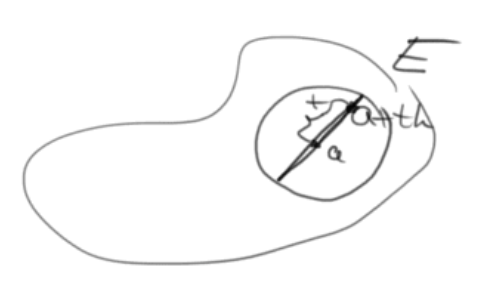
\includegraphics[width=0.2\linewidth]{images/17-05-1.png}
    \end{enumerate}
\end{remark}

\begin{theorem}
    \textbf{Экстремальное свойство градиента.}

    Пусть $f: E\rightarrow \R$, $E\subset \R^n$, $a\in \Int E$, $f$ дифференцируема в точке $a$ и $\triangledown f(a)\neq 0$. Тогда $\forall$ $h\in \R^n$ единичного $-\|\triangledown f(a)\|\leq \partialderivative{f}{h}(a) \leq \|\triangledown  f(a)\|$ и неравенство обращается в равенство $\Leftrightarrow h=\pm \frac{\triangledown f(a)}{\|\triangledown f(a)\|}$.
\end{theorem}

\begin{remark}
    Смысл: градиент задает то направление, в котором производная по направлению самая большая по модулю, то есть градиент – это направление наибыстрейшего изменения функции.
\end{remark}

\begin{proof}
    $|\frac{\partial f}{\partial h}(a)|=|\langle\triangledown f(a), h \rangle|\leq \|\triangledown f(a)\|\cdot \|h\|=\|\triangledown f(a)\|$ и неравенство Коши-Буняковского обращается в равенство $\Leftrightarrow$ вектора пропорциональны.
\end{proof}

\begin{definition}
    Пусть  $f: E\rightarrow \R$, $E\subset \R^n$, $a\in \Int E$, $f(x_1, ..., x_n)$. Тогда \textit{частной производной по $x_k$ в точке $a$} называется $\frac{\partial f}{\partial x_k}(a)=\frac{\partial f}{\partial e_k}(a)$, где $e_k=\begin{pmatrix}
        0_1 \\ \vdots \\ 0_{k-1} \\ 1_k \\ \vdots \\ 0)
    \end{pmatrix}$.

    Альтернативные обозначения: $f'_{x_k}(a)$, $ \partial_kf(a)$, $D_k f(a)$.
\end{definition}

\begin{statement}
    $\frac{\partial f}{\partial x_k}(a)=\langle \triangledown f(a), e_k\rangle$, то есть $\triangledown f(a)= (\frac{\partial f}{\partial x_1}(a), ..., \frac{\partial  f}{\partial x_n}(a))$.

    (производная по направлению – градиент скалярно умножить на направление, а частная производная – это производная по направлению $e_k$)
\end{statement}

\begin{corollary}
    Пусть $f: E\rightarrow \R^m$, $E\subset \R^n$, $a\in \Int E$ и $f$ дифференцируема в точке $a$. Тогда $f'(a)=\begin{pmatrix}
        \pdv{f_1}{x_1}(a) && \pdv{f_1}{x_2}(a) && ... && \pdv{f_1}{x_n}(a) \\
        ... && ... && ... && ... \\
        \pdv{f_m}{x_1}(a) && \pdv{f_m}{x_2}(a) && ... && \pdv{f_m}{x_n}(a)
    \end{pmatrix}$
\end{corollary}

\begin{proof}
    $f'(a)=\begin{pmatrix}
        \triangledown f_1(a) \\ \vdots \\ \triangledown f_m(a)
    \end{pmatrix}$
\end{proof}

\begin{example}
    Пусть $f(x, y)=x^y$, $x, y>0$.

    Тогда: 
    
    $\frac{\partial f}{\partial x}(a, b)=\lim\limits_{t\rightarrow 0}\frac{f(a + t, b)- f(a, b)}{t}=ba^{b-1}$

    $\frac{\partial f}{\partial y}(a, b)=\lim\limits_{t\rightarrow 0}\frac{f(a, b + t)- f(a, b)}{t}=a^b \ln a$
\end{example}

\begin{theorem}
    \textbf{Линейность дифференциала.}

    Пусть $f, g: E\rightarrow \R^m$, $E\subset \R^n$, $a\in \Int E$, $\lambda\in \R$, $f, g$ дифференцируемы в точке $a$. Тогда $f+g$ и $\lambda f$  дифференцируемы в точке $a$ и:
    
    $d_a(f+g)=d_a f+d_a g,\quad$ $(f+g)'(a)=f'(a)+g'(a)$

    $d_a(\lambda f)=\lambda\cdot  d_a f,\quad$ $(\lambda f)'(a)=\lambda f'(a)$
\end{theorem}

\begin{proof}
    $f(a+h)=f(a)+d_af(h)+\alpha (h)\| h\|$, где $\alpha (h)\underset{h\rightarrow 0}{\rightarrow}0$

    $g(a+h)=g(a)+d_ag(h)+\beta (h)\| h\|$, где $\beta (h)\underset{h\rightarrow 0}{\rightarrow}0$

    $\Rightarrow f(a+h)+g(a+h)=f(a)+g(a)+\underbrace{d_af(h)+d_ag(h)}_{\text{лин.}}+\underbrace{\alpha (h)\| h\|+\beta (h)\| h\|}_{\underset{h\rightarrow 0}{\rightarrow}0}$

    $\Rightarrow \lambda f(a+h)=\lambda f(a)+\underbrace{\lambda d_af(h)}_{\text{лин.}}+\underbrace{\lambda \alpha (h)\| h\|}_{\underset{h\rightarrow 0}{\rightarrow}0}$
\end{proof}

\begin{theorem}
    \textbf{Дифференцируемость композиции.}

    Пусть $f: D\rightarrow \R^n$, $g: E\rightarrow \R^m$, $D\subset \R^l$, $E\subset \R^n$, $a\in \Int D$ и $f(D)\subset E$. Если $f$ дифференцируема в точке $a$ и $g$ дифференцируема в точке $f(a)$, то $g\circ f$  дифференцируема в точке $a$ и $d_a(g\circ f)=d_{f(a)}g\circ d_af$, $(g\circ f)'(a)=g'(f(a))\cdot f'(a)$.
\end{theorem}

\begin{proof}
    $f(a+h) = f(a) + \underbrace{d_af(h) + \alpha (h)\|h\|}_{:=k}$, где $\alpha(h)\underset{h \rightarrow 0}{\rightarrow} 0$.

    $g(b+k) = g(b) + d_bg(k) + \beta (k)\|k\|$, где $\beta(k)\underset{k \rightarrow 0}{\rightarrow} 0$.

    Возьмем $k= d_af(h) + \alpha (h)\|h\|$. Тогда $f(a+h)=f(a)+k=b+k$.

    $g(f(a+h)) = g(b+k)=g(b)+ d_bg(k) + \beta (k)\|k\|=g(b)+d_bg(d_af(h) + \alpha (h)\|h\|)+\beta(k)\|k\|=
    g(f(a))+d_bg(d_af(h)+\underbrace{d_bg(\alpha (h)\|h\|)+\beta(k)\|k\|}_{=o(\|h\|)\ ?}$

    $d_bg(\alpha(h)\|h\|)=\|h\|d_bg(\alpha(h))$. Надо понять, что $d_bg(\alpha(h))\underset{h\rightarrow 0}{\rightarrow}0$: 
    
    $\|d_bg(\alpha(h))\|\leq \|d_bg\|\cdot \underbrace{\|\alpha(h)\|}_{\underset{h \rightarrow 0}{\rightarrow} 0}\Rightarrow$ первое слагаемое маленькое.

    Осталось понять, что $\frac{\beta(k)\|k\|}{\|h\|}\underset{h\rightarrow 0}{\rightarrow}0$: 
    
    $\|k\| =\|d_af(h)+\alpha(h)\|h\|\|\leq \|d_af(h)\|+\|\alpha(h)\|h\|\|\leq \|d_af\|\cdot \|h\|+\|\alpha(h)\| \cdot \|h\|=\|h\|\cdot(\underbrace{\|d_af\| +\| \alpha(h)\|}_{\text{огр.}})\leq C\cdot \|h\|$ (как константа + что-то $\rightarrow 0)\  \Rightarrow$ если $h\rightarrow 0$, то $k\rightarrow 0\Rightarrow \beta(k) \rightarrow 0$.

    $\|\frac{\beta(k)\|k\|}{\|h\|}\|=\frac{\|k\|}{\|h\|}\cdot \|\beta(k)\|\leq C\cdot \|\beta(k)\|\underset{k\rightarrow 0}{\rightarrow}0$ 

    В частности:
    
    $d_a(g\circ f)=d_bg\circ d_a f$

    $(g\circ f)'(a)=g'(b)\cdot f'(a)$
\end{proof}

\begin{theorem}
    \textbf{Дифференцирование скалярной и векторной функции.}

    Пусть $E\subset \R^n$, $a\in \Int E$, $\lambda: E\rightarrow \R$, $f: E\rightarrow \R^m$, $\lambda$ и $f$  дифференцируемы в точке $a$. Тогда $\lambda f$  дифференцируема в точке $a$ и $d_a(\lambda f)(h)=d_a\lambda (h)\cdot f(a) + \lambda (a) \cdot d_a f(h)$.
\end{theorem}

\begin{proof}
    $f(a+h) = f(a) + d_af(h) + \alpha (h)\|h\|$, где $\alpha(h)\underset{h \rightarrow 0}{\rightarrow} 0$.

    $\lambda(a+h) = \lambda(a) + d_a\lambda(h) + \beta (h)\|h\|$, где $\beta(h)\underset{h \rightarrow 0}{\rightarrow} 0$.
    
    $\lambda(a+h)f(a+h)=\underbrace{\overset{1}{\lambda(a)f(a)}}+
    \underbrace{\overset{2}{\lambda(a)d_af(h)}+
    \overset{3}{d_a\lambda(h)f(a)}}+$
    
    $\underbrace{\overset{4}{d_a\lambda(h)d_af(h)}+
    \overset{5}{\beta(h)\|h\|f(a)}+
    \overset{6}{\beta(h)\|h\|d_af(h)}+
    \overset{7}{\alpha(h)\beta(h)\|h\|^2}+
    \overset{8}{\lambda(a)\alpha(h)\|h\|}+
    \overset{9}{\alpha(h)\|h\|d_a\lambda(h)}}_{\overset{?}{=}o(h)}$

    $5.\ \underbrace{\beta(h)}_{\rightarrow 0}\underbrace{f(a)}_{const}\|h\|=o(\|h\|)$ 

    $8.\ \underbrace{\alpha(h)}_{\rightarrow 0}\underbrace{\lambda(a)}_{const}\|h\|=o(\|h\|)$ 

    $7.\ \underbrace{\alpha(h)\beta(h)\|h\|}_{0}\|h\|=o(\|h\|)$

    $\|d_af(h)\|\leq\|d_af\|\cdot \|h\|\underset{h\rightarrow 0}{\rightarrow}0$  и в частности ограничена.

    $\|d_a\lambda(h)\|\leq\|d_a\lambda\|\cdot \|h\|\underset{h\rightarrow 0}{\rightarrow}0$ и в частности ограничена.

    $6.\ \underbrace{\beta(h)}_{\rightarrow 0}\underbrace{d_af(h)}_{\text{огр.}}\|h\|=o(\|h\|)$

    $9.\ \underbrace{\alpha(h)}_{\rightarrow 0}\underbrace{d_a\lambda(h)}_{\text{огр.}}\|h\|=o(\|h\|)$

    $4.\ \|d_a\lambda(h)\cdot d_af(h)\|=\|d_a\lambda(h)\|\cdot\| d_af(h)\|\leq \|d_a\lambda\|\cdot\| d_af\| \cdot \|h\|^2=o(\|h\|)$
\end{proof}

\begin{theorem}
    \textbf{Дифференцирование скалярного произведения векторнозначных функций.}

    Пусть $E\subset \R^n$, $a\in \R^n$, $a\in \Int E$, $f, g:E\rightarrow \R^m$ дифференцируемы в точке $a$. Тогда $\langle f, g\rangle$  дифференцируемо в точке $a$ и $d_a\langle f, g\rangle (h)= \langle d_a f(h), g(a) \rangle + \langle f(a), d_a g(h)\rangle$. 
\end{theorem} 

\begin{proof}
    $\langle f, g\rangle =\sum\limits_{k=1}^m f_k g_k\Rightarrow \langle f, g\rangle $  дифференцируемо в точке $a$  по предыдущей теореме (как скалярные функции):

    $d_a \langle f, g\rangle (h) = \sum\limits_{k=1}^m d_a(f_kg_k)(h) =\sum\limits_{k=1}^m (d_af_k(h)g_k(a)+f_k(a)d_ag_k(h))) = \langle d_a f(h), g(a) \rangle + \langle f(a), d_a g(h)\rangle$
\end{proof}

\begin{remark}
    Если $n=1$, то формула упрощается (умножение числа на вектор): $\langle f(x), g(x) \rangle ' = \langle f'(x), g(x) \rangle  + \langle f(x), g'(x) \rangle $.
\end{remark}

\begin{theorem}
    \textbf{Теорема Лагранжа для векторнозначных функций.}

    Пусть $f: [a, b]\rightarrow \R^n$ непрерывна на $[a, b]$ и дифференцируема на $(a, b)$. Тогда $\exists c\in (a, b)$, т.ч. $ \|f(b) - f(a)\|\leq (b-a) \|f'(c)\|$.
\end{theorem}

\begin{proof}
    Возьмем $\varphi(x):=\langle f(x), f(b) - f(a)\rangle : [a, b]\rightarrow \R$  непрерывная на $[a, b]$ и дифференцируемая на $(a, b)$. Тогла по теореме Лагранжа для $\varphi$ найдется $c\in (a, b)$, т.ч. $ \varphi (b) - \varphi (a)= (b - a) \varphi '(c) = (b-a)\langle f'(c), f(b) - f(a) \rangle$.

    $\varphi(b) - \varphi (a) =\langle f(b), f(b) - f(a) \rangle - \langle f(a), f(b) - f(a) \rangle= \langle f(b)-f(a), f(b) - f(a) \rangle= \|f(b) - f(a)\|^2=(b - a)\langle f'(c), f(b) - f(a) \rangle\leq (b-a)\cdot\|f'(c)\| \|f(b) - f(a)\|$  и сократим $\|f(b) - f(a)\|$ (если был $f(b)=f(a)$, то изначальное неравенство было очевидно: справа 0, а слева что-то неотрицательное).
\end{proof}

\begin{remark}
    Равенство может никогда не достигаться.

    $f(x) = \begin{pmatrix}
        \cos x \\ \sin x
    \end{pmatrix}: [0, 2\pi ]\rightarrow \R^2\quad f(2\pi) - f(0)=\begin{pmatrix}
        0 \\ 0
    \end{pmatrix}\quad \|f(2\pi) - f(0)\|= 0$

    $f'(x) = \begin{pmatrix}
        -\sin x \\ \cos x
    \end{pmatrix}\quad \|f'(x)\|=1$
\end{remark}